\documentclass{article}
\usepackage[utf8]{inputenc}
\usepackage{xcolor}
\usepackage{graphicx}
\usepackage{wrapfig}
\usepackage{caption}
\usepackage{listings}
\usepackage{mdwlist}
\usepackage{colortbl}
\usepackage{textcomp}
\usepackage{multicol}
\usepackage{savetrees}
\usepackage{fancyhdr}
\usepackage{fancybox, graphicx}
\usepackage{shadowimage}
\usepackage{subcaption}
\usepackage{enumitem}
\usepackage{lipsum}
\providecommand\FootText{SEBI Venlo}
\setlength\parindent{0pt}
\setlength\parskip{0\baselineskip}
\setlength\headwidth{\textwidth}

\fancyhf{}
\fancyfoot[RO,LE]{\vspace{-7.5mm}
  \textbf{\Large\sf\bfseries\FootText}
}
\fancyhead[RO,LE]{Java 1}
\fancyfoot[RE,LO]{\includegraphics[width=18mm]{figures/fon000_00c.pdf}}

\renewcommand\footrule{
  \hrule height .2pt width \headwidth
}

% \fancyfoot[RE,LO]{\includegraphics[width=2cm]{figures/fon000_00c.pdf}}
% \fancyfoot[RO,LE]{\vspace{-12mm}
%   \textbf{\sf{}Fontys SEBI Venlo}
% }  

\fancyfoot[C]{\vspace{-7mm}\sffamily\bfseries\thepage}
\pagestyle{fancyplain}


\usepackage[british]{babel}
\definecolor{listinggray}{gray}{0.95}
\definecolor{lbcolor}{gray}{.95}%,0.9,0.9}
\input{pro1lstsettings}
\lstset{language=java,basicstyle={\small}}
%% to be able to use the euro sign
\usepackage{eurosym}
%% to be able to simply type the (utf-8) euro sign
\DeclareUnicodeCharacter{20AC}{\euro}
\usepackage[pdftex]{hyperref}


\title{Clock Exercise}
\author{Richard~van~den~Ham, Pieter~van~den~Hombergh\\Maximilian Walter, Ron Gebauer}
\def\Sep{\vspace{-\baselineskip}\hrulefill\vspace{-.5\baselineskip}}
\date{2015-11-06}
%% this allows the use of bar to show code in listings style 
%% like |int number = 10;|, which is nice and short.
\lstMakeShortInline|
\lstset{language=Java}
\lstset{basicstyle={\color{blue}}}
\begin{document}
\maketitle
\section*{Introduction}
This assignment is about a clock. We’ll use the clock example
extensively during the remaining part of the Java 1 course. Think about
an alarm clock you might have (had) at home.

Notice how the seventies clock shows 4 time elements: weekday, hour,
minute and second. The middle two share technology. This is the kind
of ``model'' to keep in mind when designing your own solution.
\begin{figure}[h]
  \begin{subfigure}{.6\textwidth}\centering
    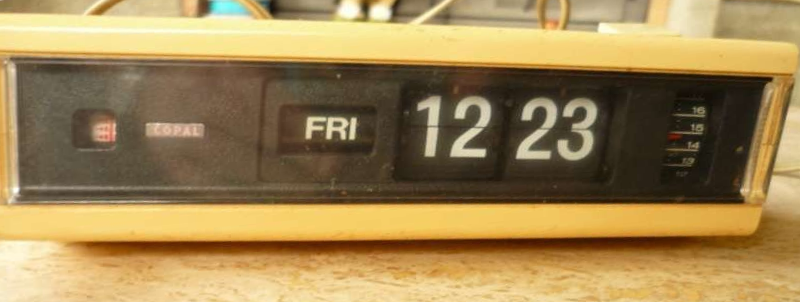
\includegraphics[width=.9\textwidth]{figures/straightseventiesclock.png}
    \caption{Seventies clock}
  \end{subfigure}
  \begin{subfigure}{.4\textwidth}\centering
    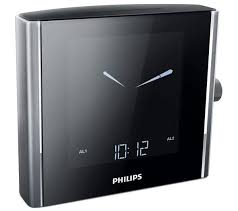
\includegraphics[width=.9\textwidth]{figures/modernclock.jpg}
    \caption{Modern LCD clock}
  \end{subfigure}
  \caption*{A small clock zoo}
\end{figure}
\begin{multicols}{2}
You’ll program a clock like this, including all its functionality and
both the digital as well as the analog display, step by step. This
assignment is the first part. {\color{red}As a starting point, study the clock
implementation described in the BlueJ book.

Note that the solution in the book is \underline{not} perfect, object orientation
wise. It is up to you to improve it.

You will refactor (to be explained) the solution in the next assignment.}
Note that the seventies clock is actually a mechanical clock, driven
by a synchronous electric motor, which drives the right hand time
element which in turn drives the element on  its left and so on.

\subsection*{Tasks}
Give the answer to the questions below in the README.txt file inside the Bluej project.
You can also take notes there, to keep things in one place.

\begin{enumerate}[label=\Alph*]
\item What are functions available in both left and right clock designs?
  \begin{itemize*}
  \item Think of display(s), buttons and what time means.
  \item Describe these functions.
  \item Is there any interaction between the elements in the display?
  \end{itemize*}
\item Describe how you would thoroughly test this physical
  machine. Use the interface of assignment A in your description.
\item Create a BlueJ project and implement a java class with the name
  |Clock| which provides the information for the display(s) in the
  clock. Understand that the clock display(s) (is/are) just a client of this
  clock class; therefore getter-methods
  and / or a |toString()| method are needed.
  Be aware that for this moment, we don’t implement a clock that is
  actually running, but just a clock that is able to register a
  certain time which we can manipulate (set, advance) manually.
\item Write a unit tests to test your clock implementation,
  based on the described script in assignment B.
\item Add seconds and days: Make sure that your clock registers days, hours,
  minutes and seconds too. Change your clock to provide this added
  functionality.
\item Consider your implementation and check if it is DRY (do not
  repeat yourselves).
\item Could you come up with better names for the classes used in the
  book clock exercise?
\end{enumerate}
\end{multicols}


\begin{multicols}{2}
\subsection*{It's time to refactor!} 

Hopefully you managed to implement the 'model' of a clock, enabling you
to store days, hours, minutes and seconds and to tick the clock manually. Your 
unit tests should have convinced you that you're ready for the next steps!


\begin{enumerate}[label=\Alph*]
\item Time to refactor! Refactoring means improving your code (e.g. design, code quality)
without adding any additional functionality. The external interface stays exactly the 
same, and therefore your unit / integration tests will still be valid. It's even so that 
refactoring without proper unit tests is an absolute NO GO!

Find a peer student (of course not the one you worked together with already during development) 
and discuss each others solutions. Make sure that your peer has about the same
programming experience / level.

Consider usage of inheritance in your new design. Realize that a week day is just
a special kind of time element, with a name. After each change, run your tests!

\item Now it's time to make the clock running. Use the Timer class in package 
javax.swing. Read the API documentation to figure out how the timer can be used.

\subsection*{What time is it?}
Congratulations! Your clock is running. Did you develop a display already? As mentioned
before, your display is a client of the actual Clock class. For the moment, a TUI (Text User 
Interface) is fine. That means a clock display class that just prints the actual clock time.
Think about a proper design to get things working!

\end{enumerate}
\end{multicols}
\Sep
\begin{multicols}{2}
\subsection*{Alarm, alarm!} 

Your clock is running! With the time, new requirements pop-up. 

\begin{enumerate}[label=\Alph*]
\item Your clock application needs to be easily extensible. Since we have to develop 
a graphical user interface (GUI) later on, we have to be prepared. The TUI and the GUI
are both listeners, listening to a clock 'model' which is doing the work. The TUI and the
GUI are so-called \textit{Observers}, since they are observing an \textit{Observable} clock.
Translate this analogy to your application. For the moment, only the TUI needs to work.

\item Stay up-to-date! Isn't it anoying to set date and time manually? Yes it is. Extend your
clock by providing functionality to set the current date / time. Figure out how to get to know
the current time using the Java Class Library.

\item Wake up, your clock needs alarm functionality. Is your clock time equal to the alarm
time? Does it ring a bell? Designing is an art.


\end{enumerate}
\end{multicols}
\Sep
\begin{multicols}{2}
\subsection*{Show it!} 

It's time to create a graphical user interface (GUI). Develop a window that shows the time
as a (J)label. Make sure that your window is an Observer of your clock. Add a button to the
window to stop the clock in case it's running, and to start the clock in case it's not yet running.
As usual, Red means stop, Green means run. Color the button accordingly.

\end{multicols}
\Sep
\begin{multicols}{2}
\subsection*{Time to finish!} 
The remaining text concludes the assignments for this semester.

Let's further extend and improve the graphical user interface
(GUI). Add the functionality below in the given order.

\begin{enumerate}[label=\Alph*]

\item Add a button that enables you to set the current (system clock) time.

\item Add  buttons to increment and decrement hours and minutes. 

\item Add a button that enables you to switch between display of
  clock~time and alarm~time. Tip: subtly adapt the |JLabel| to indicate
  which time is shown.

\item Use a Layout manager instead of placing components manually for
  the top level component. Use a |BorderLayout| as main layout. Tip:
  see the
  \href{https://docs.oracle.com/javase/tutorial/uiswing/layout/index.html}{Oracle
    tutorial on Component Layout}. The |NORTH| section shows a header text, the |CENTER| section shows the clock 
time (either actual time or alarm time).

\item (For next week...) Add a |MouseListener| to the start/stop button, that changes the 
text color to a brighter color when the mouse 'enters' the button surface and goes back
to the normal color when the mouse 'exits' the button area. The way to
work is similar to how you add an |ActionListener| to a button. 

\item Add an analog view to your clock, by drawing clock pointers for hours, minutes and 
seconds.

\item Change the visual appearance of the buttons to increment hours
  and minutes. 
  The buttons should show up or down pointing shapes. Note that
  you can add images to Buttons. The color should still change
  appearance when the mouse pointer is hovering above the button.

\end{enumerate}
\paragraph{Small steps does it.} No need to get worried. Work
step-by-step. Realize that our goal is not to get perfect and really fancy clock 
implementations; our goal is to get you to experiment with concepts, based on a 
working example. E.g. when you have to draw an analog clock-hand, 
a very first step is to draw just a line between two points. In the
second step move one of the points and draw the line again when the
|TimeElement| triggers an update. Work in small steps. Think of the
responsibilities of the classes. Keep the classes small and focused. Commit often.
\end{multicols}

\end{document}
